% Created 2022-11-08 Tue 00:49
% Intended LaTeX compiler: pdflatex
\documentclass[10pt, presentation, colorlinks]{beamer}
\usepackage[utf8]{inputenc}
\usepackage[T1]{fontenc}
\usepackage{graphicx}
\usepackage{longtable}
\usepackage{wrapfig}
\usepackage{rotating}
\usepackage[normalem]{ulem}
\usepackage{amsmath}
\usepackage{amssymb}
\usepackage{capt-of}
\usepackage{hyperref}
\usecolortheme{magpie}
\usepackage{minted}
\usemintedstyle{monokai}
\newminted{haskell}{}
\usetheme{default}
\author{Rebecca Skinner}
\date{\textit{<2022-11-08 Tue>}}
\title{Your First Haskell Terminal Application}
\subtitle{A Gentle Project-Based Introduction to Haskell}
\AtBeginSection[]{\begin{frame}<beamer>\frametitle{}\center{\huge{\secname}}\end{frame}}
\hypersetup{
 pdfauthor={Rebecca Skinner},
 pdftitle={Your First Haskell Terminal Application},
 pdfkeywords={},
 pdfsubject={},
 pdfcreator={Emacs 28.2 (Org mode 9.5.5)},
 pdflang={English}}
\begin{document}

\maketitle

\section{Prelude}
\label{sec:org4f139d7}

\begin{frame}[label={sec:org9b38032}]{Hello, World}
\begin{itemize}
\item About Me: Rebecca Skinner
\begin{itemize}
\item Lead Software Engineer at Mercury
\item Author of Effective Haskell
\end{itemize}
\item @cercerilla on Twitter and Cohost
\item \url{https://rebeccaskinner.net}
\item \url{https://github.com/rebeccaskinner/}
\end{itemize}

\begin{center}

\includegraphics[height=0.3\textheight]{img/url.png}
\end{center}
\end{frame}

\begin{frame}[label={sec:org227a721}]{About This Talk}
\begin{columns}
\begin{column}[t]{0.45\columnwidth}
\begin{center}

\includegraphics[height=0.5\textheight]{img/overview.png}
\end{center}
\end{column}

\begin{column}[t]{0.45\columnwidth}
\begin{itemize}
\item This talk is inspired by the first half of \uline{Effective Haskell}.
\item We'll focus on one happy path, there are tools and libraries that
are good but won't be covered.
\item This talk will give you a "lay of the land" but we'll leave out
some details.
\end{itemize}
\end{column}
\end{columns}
\end{frame}

\begin{frame}[label={sec:org74d4a3f}]{Effective Haskell}
\begin{columns}
\begin{column}[t]{0.45\columnwidth}
\begin{center}
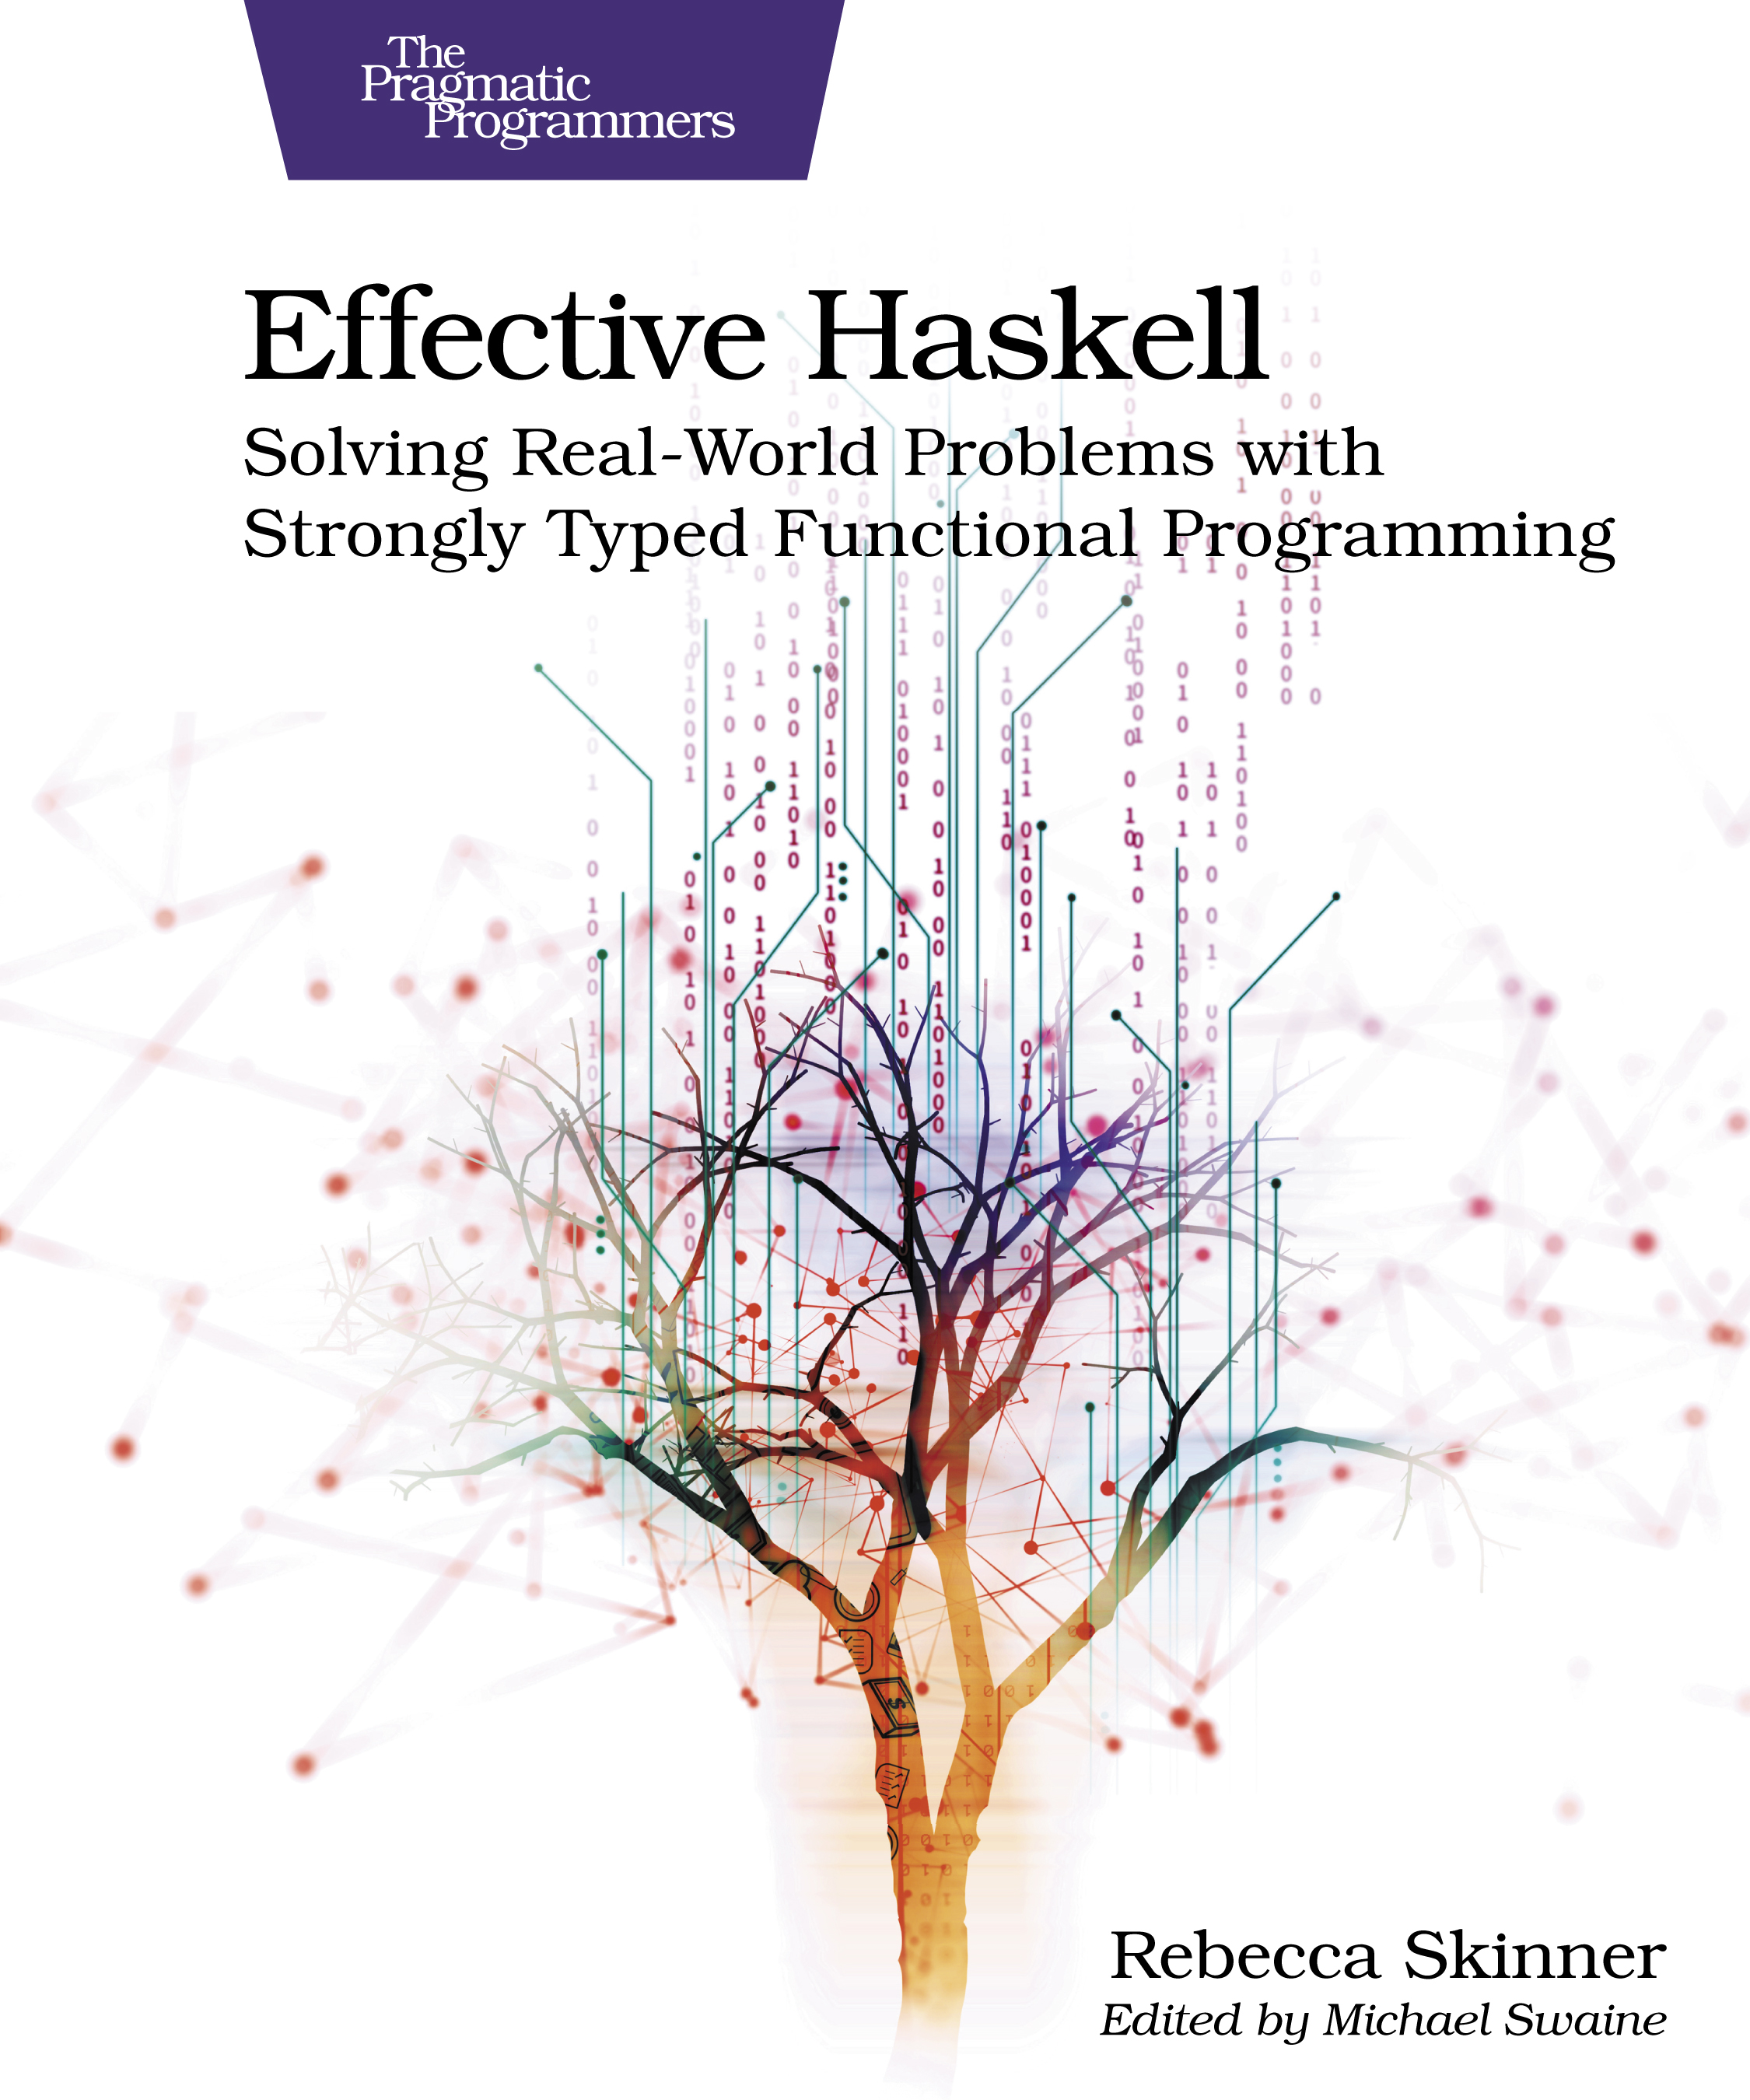
\includegraphics[height=0.7\textheight]{img/rshaskell.jpg}
\end{center}
\end{column}

\begin{column}[t]{0.45\columnwidth}
\begin{figure}[htbp]
\centering

\includegraphics[height=0.3\textheight]{img/effective-haskell-url.png}
{\tiny{https://tinyurl.com/2744kfu7\\ Now in Beta!}}
\end{figure}
\end{column}
\end{columns}
\end{frame}

\section{Build Your Tools!}
\label{sec:org41e8e2d}

\begin{frame}[label={sec:org2b3a077}]{Build Your Tools!}
\begin{center}

\includegraphics[height=0.7\textheight]{img/build-your-own-tools.png}
\end{center}
\end{frame}

\begin{frame}[label={sec:org7d66774}]{HCat: A Haskell Pager}
A \alert{pager} is a command line tool that lets you view long documents one
page at a time. Some examples you might be familiar with incldue:

\pause
\begin{itemize}
\item less
\item more
\item bat
\end{itemize}
\pause

We're going to build our own pager in Haskell. I'm calling mine \alert{hcat}.
\end{frame}

\begin{frame}[label={sec:org3a195e2}]{HCat: A Screenshot}
\begin{center}
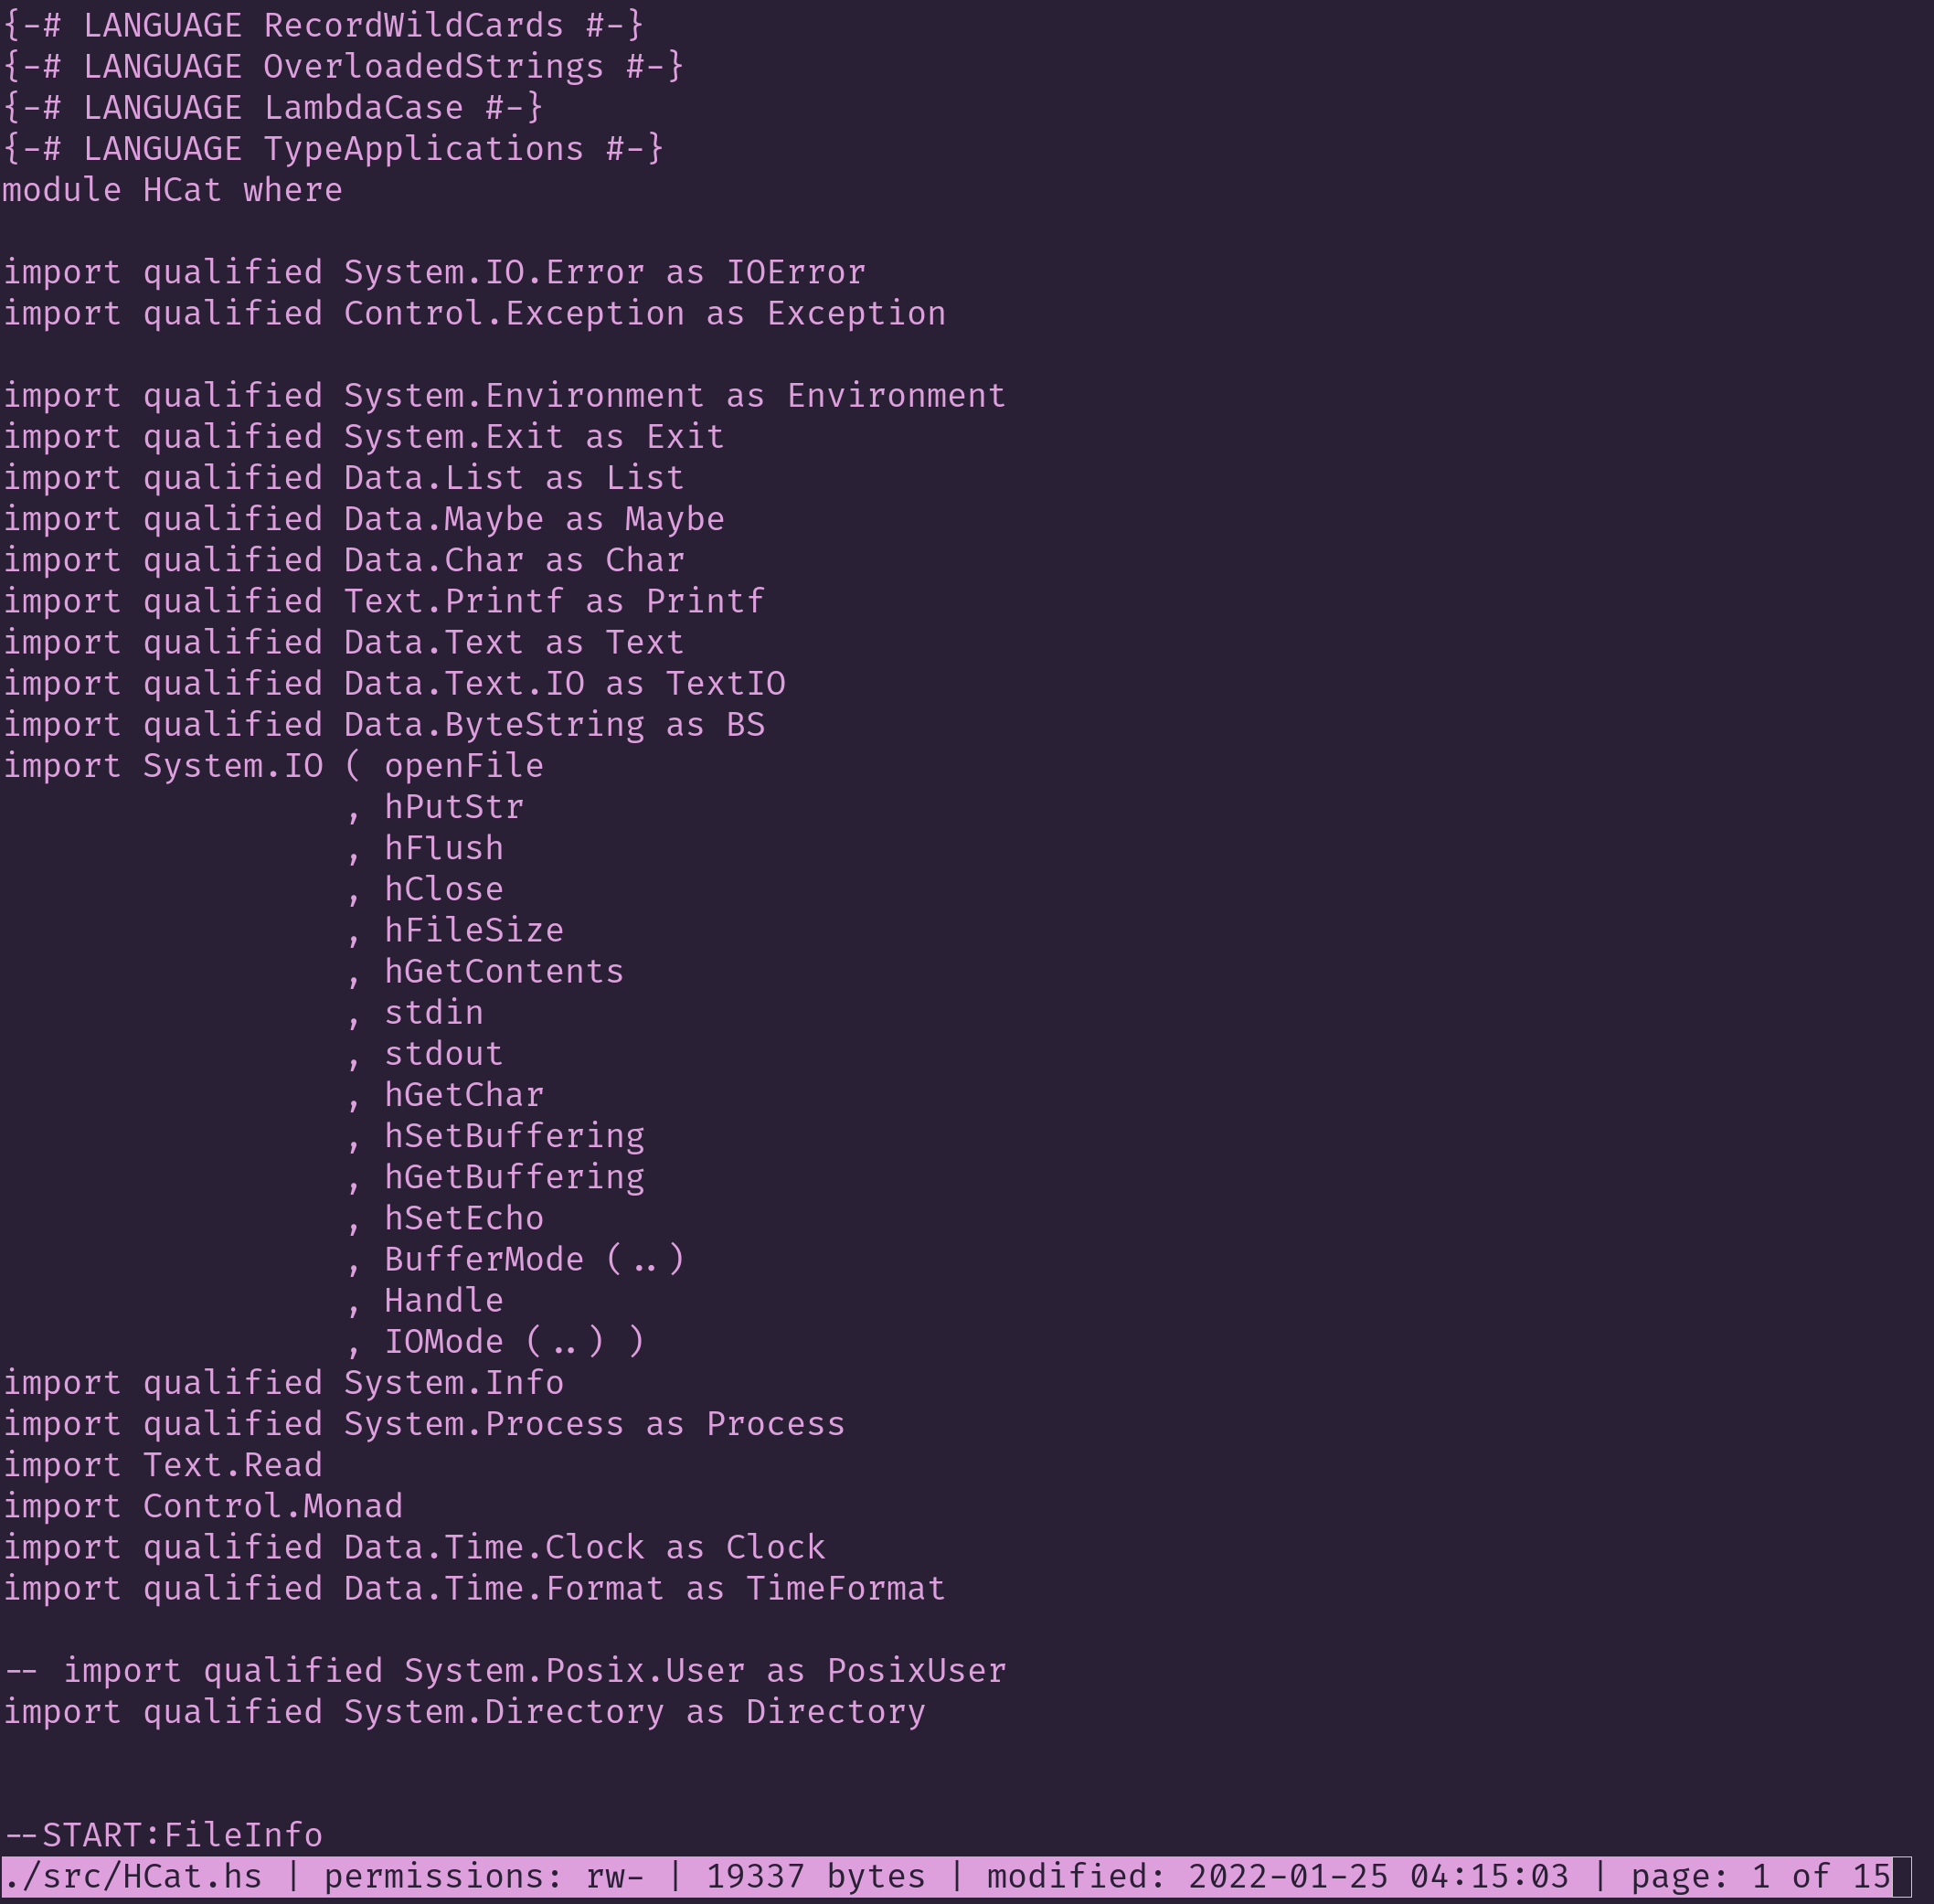
\includegraphics[height=0.8\textheight]{img/hcat-screen.png}
\end{center}
\end{frame}

\begin{frame}[label={sec:org27d8f13}]{Re-Inventing a Thousand Wheels}
Why write something boring like a pager?

\pause
\begin{itemize}
\item Teaches you how to do basic IO and work with the local system
\end{itemize}
\pause
\begin{itemize}
\item Implementing word wrap and pagination will help you think about problems in a functional way
\end{itemize}
\pause
\begin{itemize}
\item Building something similar to tools you use ever day will help you make good decisions, and give you something you can benefit from
\end{itemize}
\end{frame}

\begin{frame}[label={sec:orga65aba3}]{Choosing Haskell for Developer Tooling}
Why choose \alert{Haskell} to build your developer tooling?

\pause
\begin{itemize}
\item You want to learn Haskell, and building things for yourself is a good way to learn
\item Haskell is a compiled language, so you don't have to deal with the startup times of a JIT language like Java
\item Haskell is garbage collected (fewer memory errors)
\item Haskell is \alert{statically typed} so you'll have fewer runtime errors
\item Haskell has good performance
\begin{itemize}
\item Frequently, but not always slower than C and C++ programs
\item About as fast as Java programs while using a bit less memory, and having no JIT warmup cost
\item Nearly always faster than Python programs
\end{itemize}
\end{itemize}
\end{frame}

\section{Setting Up Your Environment}
\label{sec:orga43ecd8}

\begin{frame}[label={sec:org1e2ff38}]{Setting Up Your Environment}
\begin{center}
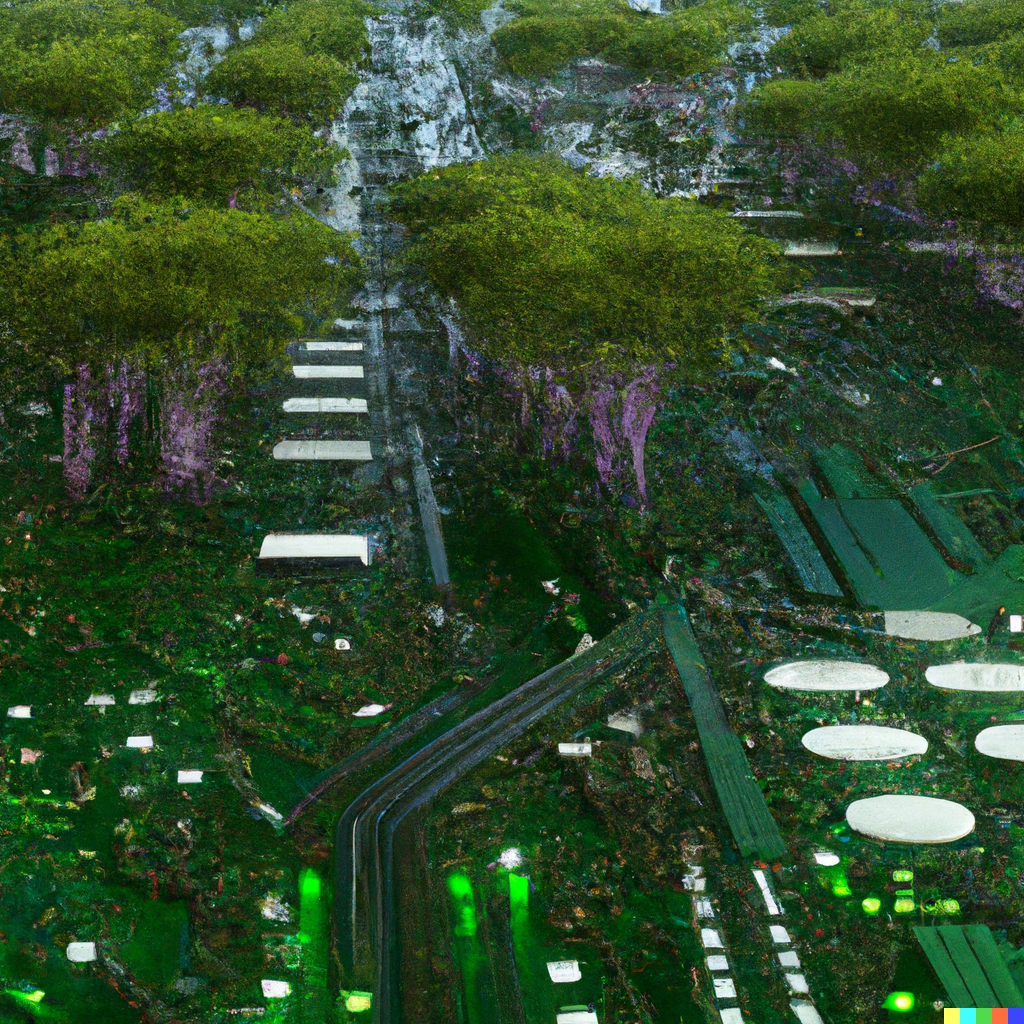
\includegraphics[height=0.8\textheight]{img/environment.png}
\end{center}
\end{frame}

\begin{frame}[label={sec:org168b8eb}]{Operating System}
Haskell works on all of the major operating systems.

\begin{itemize}
\item Linux
\begin{itemize}
\item x86 and arm. Best on x86
\end{itemize}
\item macOS
\begin{itemize}
\item Intel and Apple hardware are well supported
\end{itemize}
\item Windows
\begin{itemize}
\item x86. Native and WSL supported, but best with WSL.
\end{itemize}
\end{itemize}

\pause
I use NixOS. Haskell works great with NixOS, but it's a steep learning curve.
\end{frame}

\begin{frame}[label={sec:orgb1989e1}]{Operating System}
\begin{center}
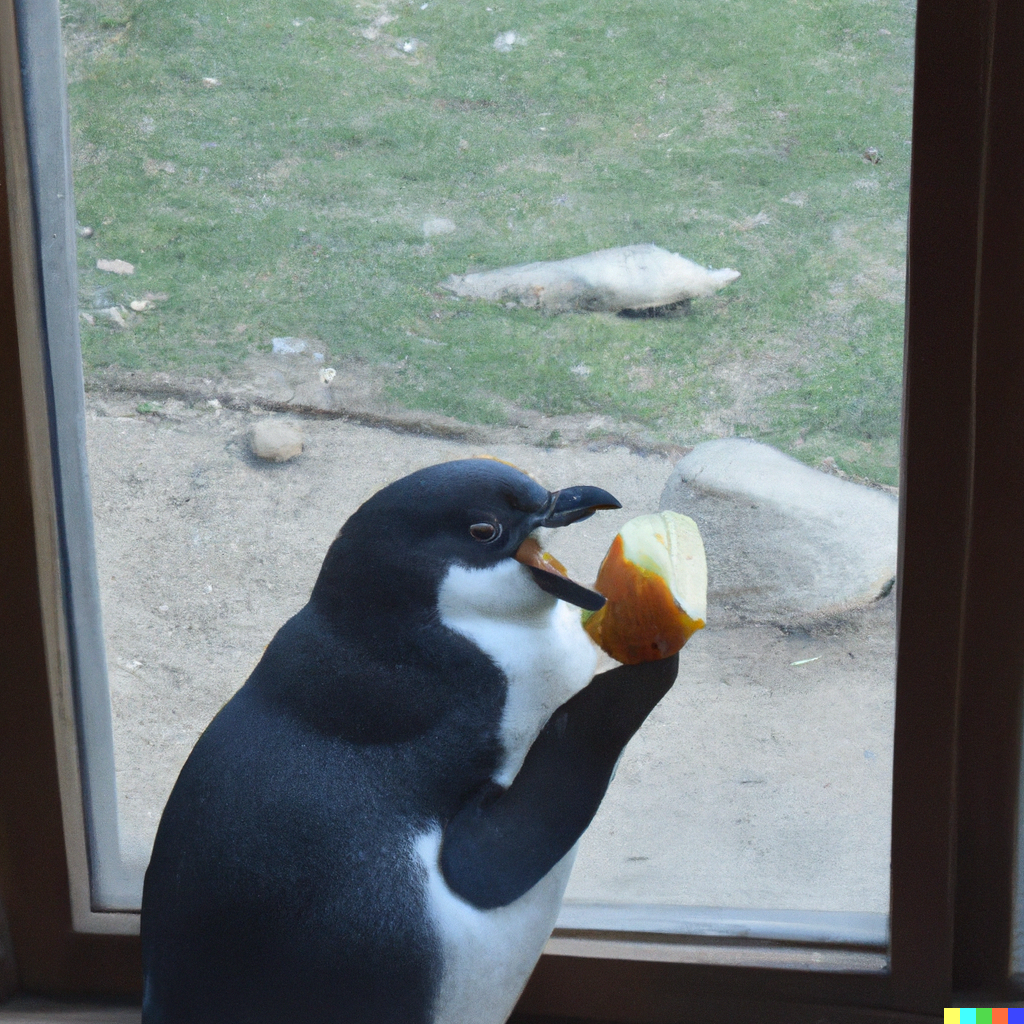
\includegraphics[height=0.5\textheight]{img/windows.png}
\end{center}
\end{frame}

\begin{frame}[label={sec:org191dc1e}]{Installing Haskell}
The best way to install Haskell is with ghcup:

\url{https://www.haskell.org/ghcup/}

\pause

\begin{itemize}
\item Managing Haskell with nixpkgs works well, but is a steep learning curve.
\item Avoid using linux distro packages, homebrew, etc.
\item Installing Haskell with Stack is no longer recommended, but you can install stack with ghcup if you like.
\end{itemize}
\end{frame}

\begin{frame}[label={sec:orgc645316}]{Configuring Your Editor}
VSCode is the most popular editor for working with Haskell. It will
help you set up additional tooling and offers the most IDE-like
experience.

Emacs and vim also have good Haskell support, and can be configured
with more IDE like features if you want.
\end{frame}

\begin{frame}[label={sec:org07152c1}]{Linting}
\alert{hlint} is the most popular Haskell linter by far. You should try to use hlint when you are developing.

\begin{itemize}
\item hlint will sometimes tell you things that you might not have learned yet, try not to worry about that too much.
\item hlint sometimes makes bad suggestions, but most of the time it's suggestions are good and will help you learn to write better Haskell programs.
\item hlint is very configurable, so you can tune it if there are things that you find annoying.
\end{itemize}
\end{frame}

\begin{frame}[label={sec:orge9a396e}]{Pretty Printing}
There are a lot of different pretty printers for Haskell. None of them
do a perfect job, and they'll all make your code worse on occasion, so
you should treat them as a tool to help you format your code, rather
than something that should be enforced.

\pause
\begin{itemize}
\item Fourmolu is modestly configurable, and tends to work reliably. It's also fairly aggressive and is more likely to uglify your code.
\item Stylish Haskell tends to lag a bit in supporting newer GHC versions, and can be a little flaky, but is less intrusive and it's style is a bit more idiomatic to classic haskellers
\end{itemize}
\pause

There are a bunch of other options you can explore if you want
\end{frame}

\begin{frame}[label={sec:orgf26fc3a}]{Too Much Text}
\begin{center}
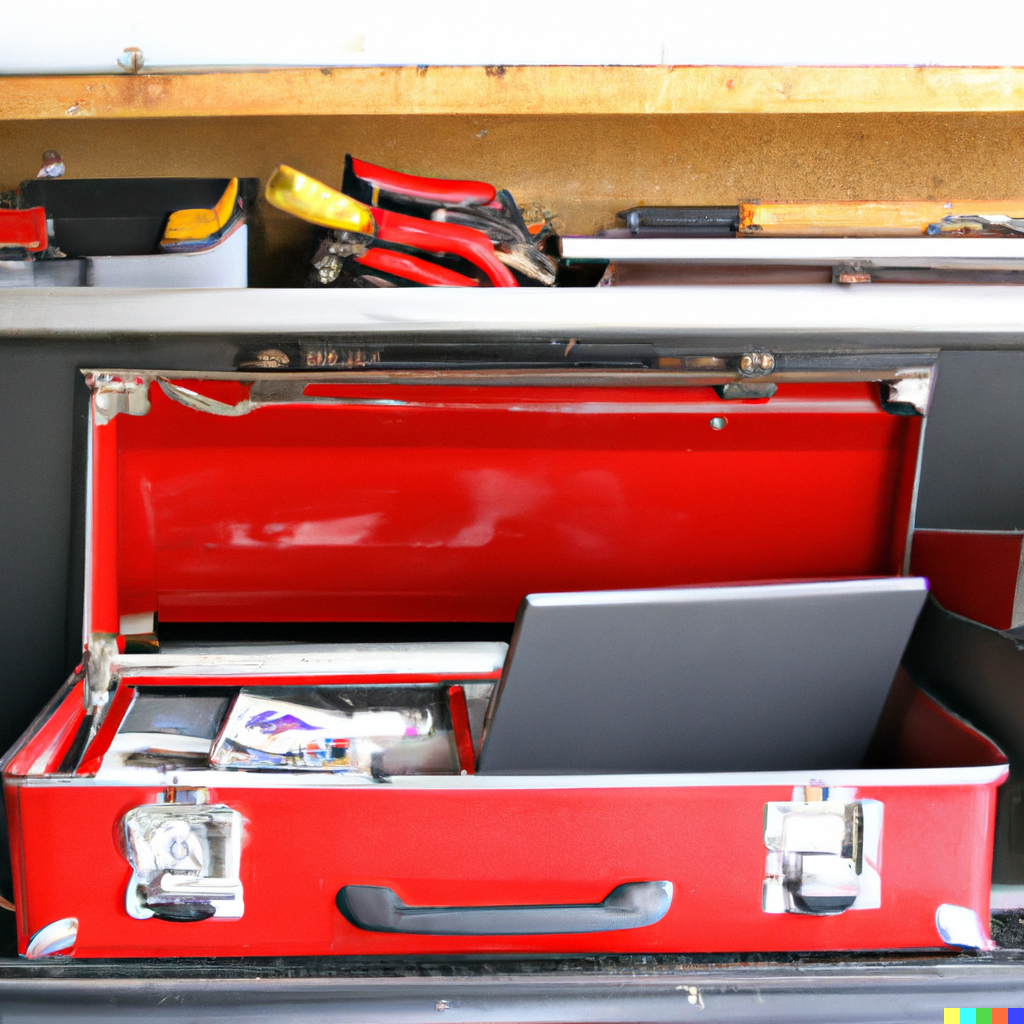
\includegraphics[height=0.8\textheight]{img/tools.png}
\end{center}
\end{frame}

\begin{frame}[label={sec:org5703c01}]{IDEs and Not-IDEs}
The Haskell Language Server (HLS) provides the most IDE-like experience for working with Haskell. Other tools you might like are:

\begin{description}
\item[{ghci}] The GHC REPL
\item[{ghcid}] The ghci repl as a deamon, with some extra features
\item[{halfsp}] A minimal Haskell language server with good performance
\item[{haskell-mode}] Emacs major mode with good REPL integration
\item[{hasktags}] ctags and etags support for navigating files
\end{description}
\end{frame}

\begin{frame}[label={sec:orgb7f03ec}]{Picking a GHC Version}
\begin{itemize}
\item As a rule of thumb, staying one version behind the newest release is a
\end{itemize}
safe strategy for getting new features in a timely manner while
avoiding broken packages.

\begin{itemize}
\item Tools tend to take longer to update than libraries, so if you are
\end{itemize}
flexible about what tools you want you can typically upgrade sooner.
\end{frame}

\section{Getting Help}
\label{sec:org3353417}

\begin{frame}[label={sec:org8b43b33}]{Browse Documentation on Hackage}
\url{https://hackage.haskell.org}

\begin{description}
\item[{Hot Tip}] When browsing documentaiton the \alert{s} key to bring up a box
that will let you search for functions by name or type
\item[{Hot Tip}] The \alert{source} links take you to a page where you can
browse the source of packages. The source is typically \alert{hyperlinked}
to source in other packages, so you can follow definitions to other
code from your browser
\item[{Hot Tip}] In search engines like DuckDuckGo and Kagi you can use
\alert{!hackage <package>} to search for a package.
\end{description}
\end{frame}

\begin{frame}[label={sec:org65fdc3c}]{Browse Documentation on Hackage}
\url{img/hackage-demo.webm}
\end{frame}

\begin{frame}[label={sec:org94af0ef}]{Search Libraries with Hoogle}
\url{img/hoogle-demo.webm}
\end{frame}

\section{Starting a New Project}
\label{sec:orgc75eae7}

\begin{frame}[label={sec:org52fd736}]{Starting a New Project}
\begin{center}
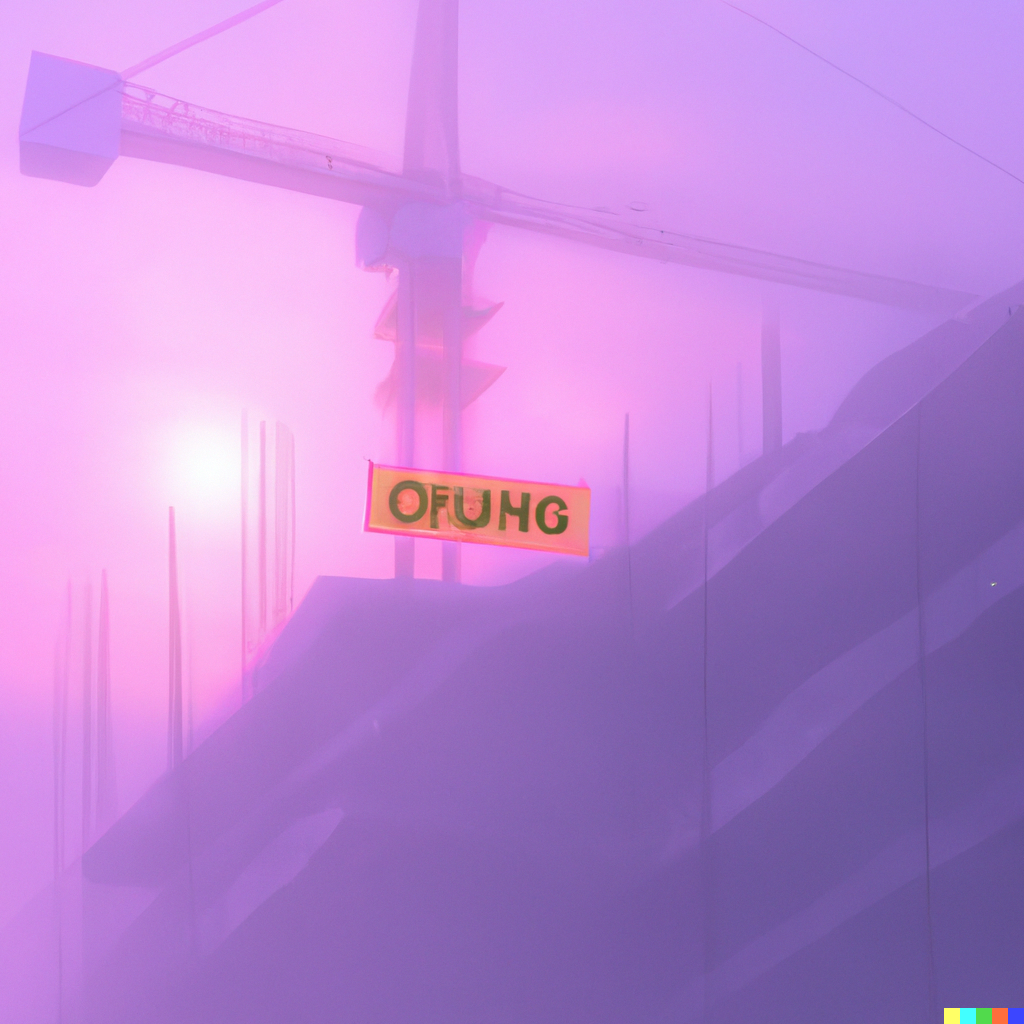
\includegraphics[height=0.8\textheight]{img/project.png}
\end{center}
\end{frame}

\begin{frame}[label={sec:org818179a},fragile]{Haskell Packaging Overview}
 You can write, build, and run a Haskell program without any special build tools:

\begin{minted}[frame=lines,fontsize=\scriptsize,linenos=false]{shell}
ghc Hello.hs && ./Hello
\end{minted}

\pause

Usually you want to use a tool like \alert{cabal} to make it easier to
manage dependencies, build your program, and run tests.
\end{frame}

\begin{frame}[label={sec:org3d8a217}]{Picking a Build Tool}
There are three popular ways to build Haskell programs:

\pause

\begin{description}
\item[{cabal}] The default tool for building packages with GHC.
\item[{stack}] Another popular tool. It aims to make dependency management easier.
\item[{nix}] Uses cabal under the hood. Provides reproducibility.
\end{description}

\pause

\alert{cabal} is a good default choice and we'll stick with it in this talk.
\end{frame}

\begin{frame}[label={sec:orgf67ba1d},fragile]{Cabal Basics}
 \begin{description}
\item[{\texttt{cabal init}}] Start a new project
\item[{\texttt{cabal build}}] Compiler your project
\item[{\texttt{cabal exec}}] Run your project
\item[{\texttt{cabal repl}}] Load your code into an interactive environment
\end{description}
\end{frame}

\begin{frame}[label={sec:orgab51906},fragile]{The Cabal File}
 \begin{minted}[frame=lines,fontsize=\scriptsize,linenos=false]{haskell-cabal}
cabal-version:       2.4
name:                hcat
version:             0.1.0.0

library
  hs-source-dirs:      src
  exposed-modules:     HCat
  build-depends:       base, bytestring, text
                     , process, directory, time
  default-language:    Haskell2010

executable hcat
  hs-source-dirs:      app
  main-is:             Main.hs
  build-depends:       base, hcat
  default-language:    Haskell2010
\end{minted}
\end{frame}

\begin{frame}[label={sec:org741202e},fragile]{App, Src, and Test}
 \begin{itemize}
\item Most haskell applications have a very minimal application. Often, the executable is a single file named \texttt{Main.hs}
\item The application logic is typically all in a library that lives in the same project along with the executable
\item Unit tests are in a \texttt{test} directory and cover the library code
\end{itemize}
\end{frame}

\begin{frame}[label={sec:orge48dceb}]{Managing Dependencies}
Don't worry too much about things like version boundaries when you are
just getting started. Focus on writing programs using only a few
popular libraries, and stick with the defaults where you can. You'll
need to be more careful in the future, but for now it's not worth
being concerned with.
\end{frame}

\section{Putting the M in MVP}
\label{sec:orgee276a1}

\begin{frame}[label={sec:orgd2acce2},fragile]{Read File, Write File}
 Haskell can look a lot like other languages you might have seen. Here's a working version of \alert{hcat}:

\begin{minted}[frame=lines,fontsize=\scriptsize,linenos=false]{haskell}
getFileNameFrom arguments = do {
  when (length arguments <= 0) do {
    fail "empty args";
  };
  return (head arguments);
}

main = do {
  arguments <- getArgs;
  fileName <- getFileNameFrom arguments;
  fileContents <- readFile fileName;
  putStr fileContents;
  return ();
}
\end{minted}
\end{frame}

\begin{frame}[label={sec:org4fe1cae},fragile]{Read File, Write File}
 But this is another working version:

\begin{minted}[frame=lines,fontsize=\scriptsize,linenos=false]{haskell}
main = getArgs >>= readFile . head >>= putStr
\end{minted}

\pause

Programs you read are more likely to look like this example than the previous one.
\end{frame}

\begin{frame}[label={sec:org486e1d3}]{Read File, Write File}
The lesson:

\pause

When you are first getting started, don't worry too much about
idiomatic code. Haskell has a lot of ways to do things, and the
learning curve is a little steep at first. Focus on getting things
working even if they aren't the "right way". Refactor as you learn
more.
\end{frame}

\begin{frame}[label={sec:orgea99345}]{Zoom, Enhance, Refactor}
\begin{center}
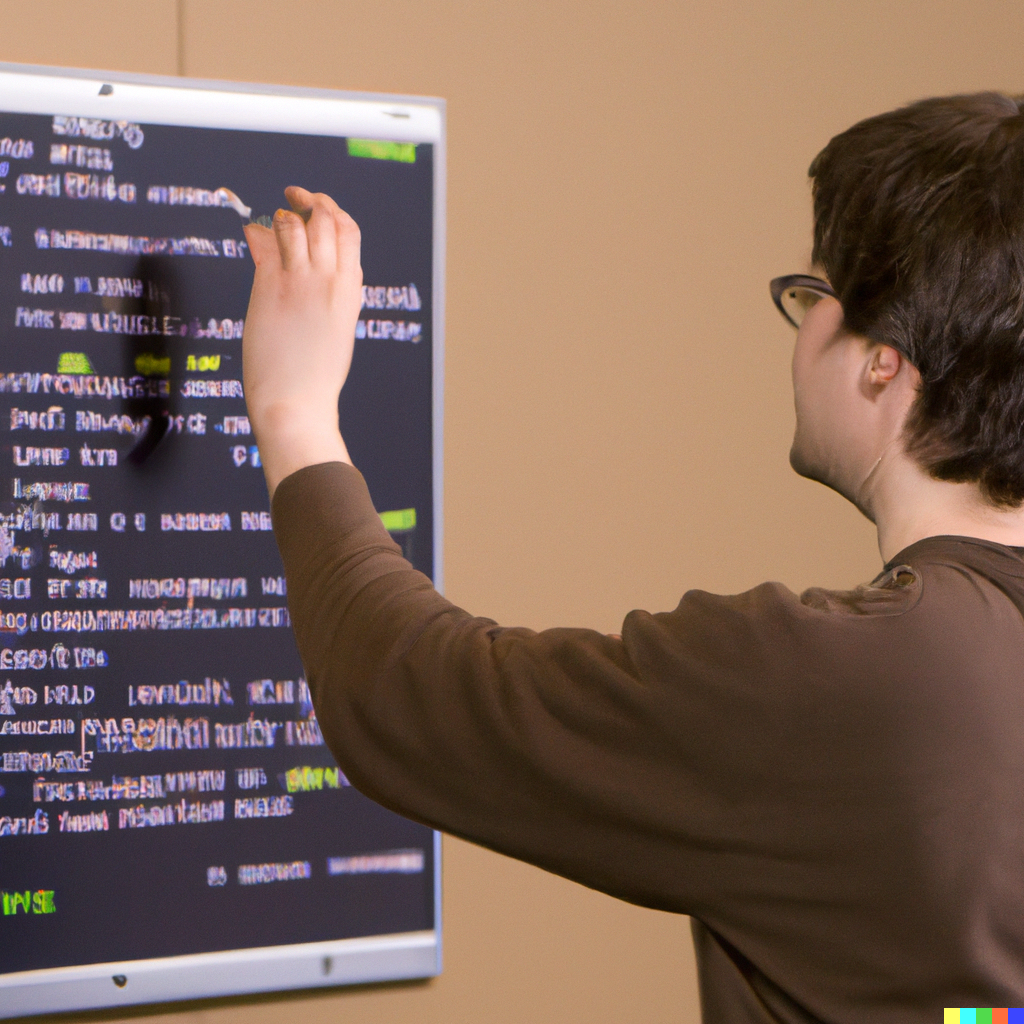
\includegraphics[height=0.8\textheight]{img/refactoring.png}
\end{center}
\end{frame}

\begin{frame}[label={sec:org76c50f1},fragile]{Zoom, Enhance, Refactor}
 Let's give this another shot. How might a reasonable version of our program look?

\pause

\begin{minted}[frame=lines,fontsize=\scriptsize,linenos=false]{haskell}
module HCat where
import System.Environment (getArgs)

filenameArgument :: IO FilePath
filenameArgument = do
  allArguments <- getArgs
  case allArguments of
    [fileName] ->
      pure fileName
    _otherwise ->
      fail "Please provide one file name"

hcat :: IO ()
hcat = do
  fileName <- filenameArgument
  fileContents <- readFile fileName
  putStr fileContents
\end{minted}
\end{frame}


\section{That's No Moon: Working With IO}
\label{sec:org9025e6b}

\begin{frame}[label={sec:org873817e}]{A Tale of Two Languages}
At first glance, our first hcat implementation seems straightforward,
but writing your first Haskell program that does substantial IO can be
tricky.
\end{frame}

\begin{frame}[label={sec:orgb43ca3a},fragile]{A Tale of Two Languages}
 \begin{columns}
\begin{column}[t]{0.45\columnwidth}
\begin{block}{In this function we're only using \alert{let} and \alert{in}}
\begin{minted}[frame=lines,fontsize=\scriptsize,linenos=false]{haskell}
reverseSentence sentence =
  let
    wordsInReverse =
      reverse (words sentence)
  in unwords wordsInReverse
\end{minted}
\end{block}
\end{column}

\begin{column}[t]{0.45\columnwidth}
\begin{block}{But in this function, we're also using \alert{do} and \alert{<-}}
\begin{minted}[frame=lines,fontsize=\scriptsize,linenos=false]{haskell}
printSentenceBackwards = do
  sentence <- getLine
  let
    reversed =
      reverseSentence sentence
  putStrLn reversed
\end{minted}
\end{block}
\end{column}
\end{columns}
\end{frame}

\begin{frame}[label={sec:org67adecd},fragile]{A Tale of Two Languages}
 \begin{columns}
\begin{column}[t]{0.45\columnwidth}
\begin{block}{This is a \alert{pure function}}
\begin{minted}[frame=lines,fontsize=\scriptsize,linenos=false]{haskell}
reverseSentence :: String -> String
reverseSentence sentence =
  let
    wordsInReverse =
      reverse (words sentence)
  in unwords wordsInReverse
\end{minted}
\end{block}
\end{column}

\begin{column}[t]{0.45\columnwidth}
\begin{block}{This is an \alert{IO Action}}
\begin{minted}[frame=lines,fontsize=\scriptsize,linenos=false]{haskell}
printSentenceBackwards :: IO ()
printSentenceBackwards = do
  sentence <- getLine
  let
    reversed =
      reverseSentence sentence
  putStrLn reversed
\end{minted}
\end{block}
\end{column}
\end{columns}
\end{frame}

\begin{frame}[label={sec:org343e624}]{We put code in your code}
An \alert{IO Action} is a \uline{program} that will be executed by the Haskell
runtime when a user launches the program. All executable Haskell
programs ultimately work by running a single IO action named \alert{main}.

\pause

\bigskip

Haskell is a pure functional language that we can use to write impure
effectful programs in the \alert{IO Action} language:

\pause

\bigskip

\begin{itemize}
\item Writing IO programs that run pure functional code
\item Creating new IO programs by running one right after another
\item Runing one IO program and passing it's output in as the input to another IO program
\item Writing an IO program that executes many other IO programs as it runs
\end{itemize}
\end{frame}

\begin{frame}[label={sec:org4297879}]{How \alert{do} you \alert{do} it?}
Haskell's \alert{do notation} gives us special syntax for working with
things like IO actions. You can think of a \alert{do block} as special
syntax to \uline{embed a program written in the IO Action language} directly
into your pure functional program. You can even \uline{interleave} pure
functional Haskell code with code written in the IO Action language.
\end{frame}

\begin{frame}[label={sec:org91a3373},fragile]{How \alert{do} you \alert{do} it?}
 Code inside of \alert{do} blocks can really look a lot like impure
procedural programming languages. Let's look at an example from
\uline{Effective Haskell}:

\bigskip

\begin{minted}[frame=lines,fontsize=\scriptsize,linenos=false]{haskell}
editDistance :: Text -> Text -> Int
editDistance stringA stringB = runST $ do
  let
    aLen = T.length stringA
    bLen = T.length stringB
    as = zip [1..] (T.unpack stringA)
    bs = zip [1..] (T.unpack stringB)
    lookupIndex x y = (y * (aLen + 1)) + x
  cache <- MVec.new $ (aLen + 1) * (bLen + 1)
  for_ [0..aLen] $ \idx -> MVec.write cache (lookupIndex idx 0) idx
  for_ [0..bLen] $ \idx -> MVec.write cache (lookupIndex 0 idx) idx
  for_ as $ \(idxA, charA) -> do
    for_ bs $ \(idxB, charB) -> do
      let
        editCost = if charA == charB then 0 else 1
      insertCost <- (1 +) <$> MVec.read cache (lookupIndex (idxA - 1) idxB)
      deleteCost <- (1 +) <$> MVec.read cache (lookupIndex idxA (idxB - 1))
      swapCost   <- (editCost +) <$> MVec.read cache (lookupIndex (idxA - 1) (idxB - 1))
      MVec.write cache (lookupIndex idxA idxB) $ min swapCost (min insertCost deleteCost)
  MVec.read cache $ lookupIndex aLen bLen
\end{minted}
\end{frame}

\begin{frame}[label={sec:org7a4cbf1}]{Slings and Arrows}
It's important to remember that things “inside” of an IO Action \uline{don't
really exist yet} when you are writing pure functional code. They
won't exist until the IO Action is run. When an IO Action program runs
and returns a value, you can't use that value in your pure code
because it hasn't been computed yet.

\pause
\bigskip
But\ldots{}..
\pause
\bigskip

IO Action programs are regular values, and you \uline{can} return them, and
work with them like any other kind of value.
\end{frame}

\begin{frame}[label={sec:org9867486},fragile]{Slings and Arrows}
 \begin{minted}[frame=lines,fontsize=\scriptsize,linenos=false]{haskell}
aBunchOfPrintStatements :: Int -> [IO ()]
aBunchOfPrintStatements count =
  [print x | x <- [0..count]]

printTenTimes :: IO ()
printTenTimes =
  for_ (aBunchOfPrintStatements 10) $ \statement -> do
    putStrLn "running a statement..."
    statement
\end{minted}
\end{frame}

\section{Putting It All Together}
\label{sec:org5d5a147}

\begin{frame}[label={sec:org9f9f494}]{Putting It All Together}
\begin{center}
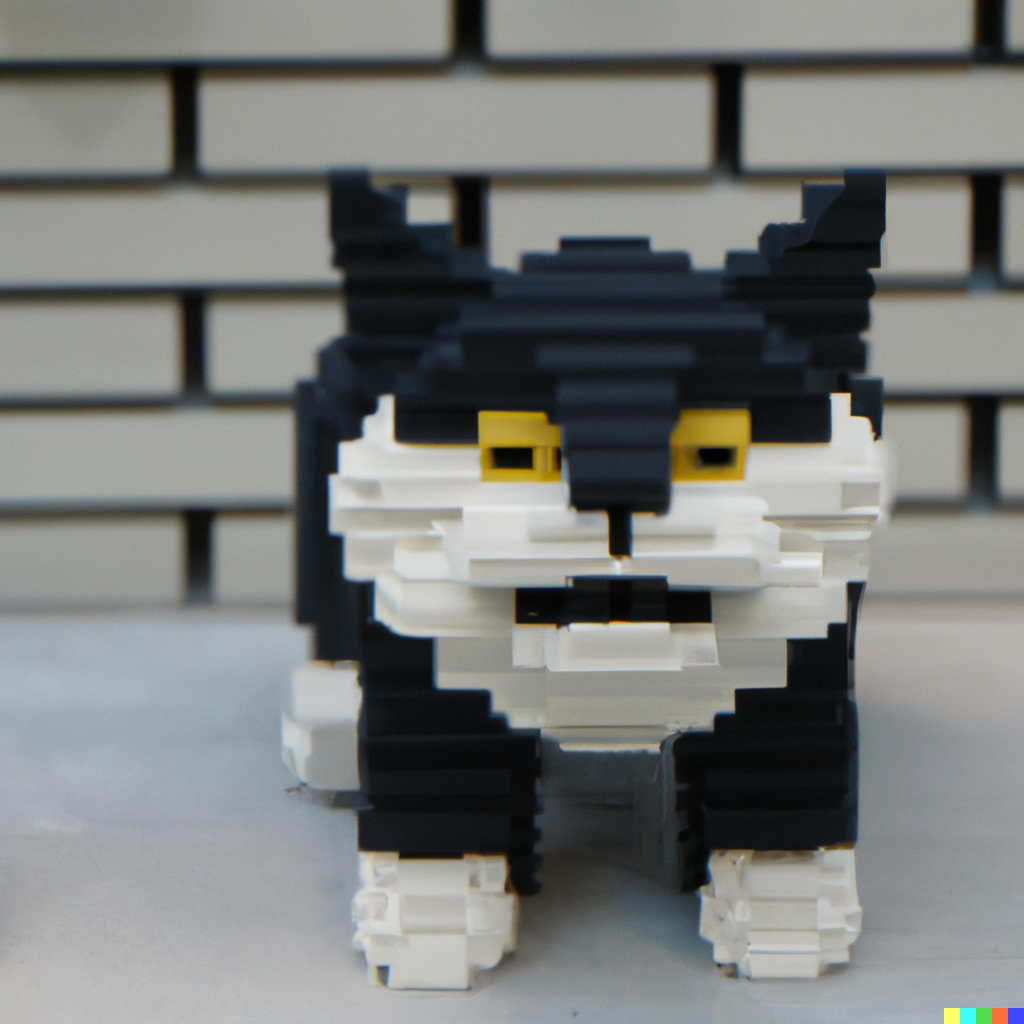
\includegraphics[height=0.5\textheight]{img/cat.png}
\end{center}
\end{frame}

\begin{frame}[label={sec:orgcbcdd43},fragile]{Putting It All Together}
 \begin{minted}[frame=lines,fontsize=\scriptsize,linenos=false]{haskell}
runHCat :: IO ()
runHCat = do
  targetFilePath <- handleArgs
  contents <- TextIO.readFile targetFilePath
  termSize <- getTerminalSize
  hSetBuffering stdout NoBuffering
  finfo <- fileInfo targetFilePath
  let pages = paginate termSize finfo contents
  showPages pages
\end{minted}
\end{frame}

\section{Questions?}
\label{sec:orgd923891}
\end{document}